\documentclass{beamer}

% ---------- Core packages (한 번씩만) ----------
\usepackage[absolute,overlay]{textpos} % textblock*
\usepackage{xcolor}
\usepackage{kotex}
\usepackage{mathtools}  % (amsmath 포함)
\usepackage{amssymb}
\usepackage{stmaryrd}
\usepackage{physics}
\usepackage{anyfontsize}
\usepackage{comment}
\usepackage{bbold}
\usepackage{varwidth}
\usepackage{lipsum}
\usepackage{mwe}



% floats/captions (원래 사용 유지)
\usepackage{caption}
\usepackage{subcaption}

% algorithm & listings (중복 제거)
\usepackage{algorithm}
\usepackage{algpseudocode}
\usepackage{listings}

% references (원래 사용 유지)
\usepackage{zref}
\usepackage{zref-user}
\usepackage{zref-xr}

% tcolorbox (원래 로드 + theorems/listings 스킨만 추가)
\usepackage{tcolorbox}
\tcbuselibrary{listings,skins,breakable,theorems}

% TikZ
\usepackage{tikz-cd}
\usepackage{tikz}
\usetikzlibrary{calc} % <-- 필수 (라벨 폭 계산)
\usetikzlibrary{arrows,shapes,positioning,shapes.geometric}

% ---------- Theme ----------
\usetheme{CambridgeUS}

% ---------- Colors ----------
\definecolor{Sogang}{rgb}{0.65234375,0.12890625,0.09375}
\definecolor{examplecolor}{rgb}{0.65234375,0.12890625,0.09375}

% global canvas
\setbeamercolor{background canvas}{bg=white}
\setbeamercolor{normal text}{fg=black,bg=white}

% structure
\usecolortheme[named=Sogang]{structure}
\setbeamercolor{frametitle}{fg=Sogang}
\setbeamercolor{title}{fg=Sogang}
\setbeamercolor{item}{fg=Sogang}

% blocks with shadow (원래 설정 유지)
\setbeamertemplate{blocks}[rounded][shadow=true]
\setbeamercolor{block title}{fg=white,bg=Sogang}
\setbeamercolor{block body}{fg=black,bg=white}
\setbeamercolor{block title example}{fg=white,bg=Sogang!85}
\setbeamercolor{block body example}{fg=black,bg=white}
\setbeamercolor{block title alerted}{fg=white,bg=Sogang!80!black}
\setbeamercolor{block body alerted}{fg=black,bg=white}
\setbeamercolor{shadow}{bg=Sogang!40!black}

% ---------- Footline (원래 템플릿 유지) ----------
\setbeamertemplate{footline}{
  \leavevmode%
  \hbox{%
    \begin{beamercolorbox}[wd=.4\paperwidth,ht=2.25ex,dp=1ex,center]{author in head/foot}%
      \usebeamerfont{author in head/foot}\insertshortauthor
    \end{beamercolorbox}%
    \begin{beamercolorbox}[wd=.6\paperwidth,ht=2.25ex,dp=1ex,center]{title in head/foot}%
      \usebeamerfont{title in head/foot}\insertshorttitle\hspace*{3em}
      \insertframenumber{} / \inserttotalframenumber\hspace*{1ex}
    \end{beamercolorbox}%
  }%
  \vskip0pt%
}

% ---------- Beamer templates ----------
\setbeamertemplate{navigation symbols}{}
\setbeamertemplate{frametitle continuation}{}
\setbeamertemplate{itemize item}{$\blacksquare$}
\setbeamertemplate{itemize subitem}{$\blacktriangleright$}
\setbeamertemplate{itemize subsubitem}{$\bullet$}
\setbeamertemplate{theorems}[numbered]
\setbeamertemplate{sections/subsections in toc}[square]
\setbeamertemplate{caption}[numbered]

% ---------- Listings ----------
\lstset{
  language=Python,
  basicstyle=\ttfamily\small,
  breaklines=true,
  showstringspaces=false,
  keywordstyle=\color{blue},
  commentstyle=\color{green!50!black},
  stringstyle=\color{orange},
  numbers=left,
  numberstyle=\tiny\color{gray},
  frame=single,
  rulecolor=\color{black},
  captionpos=b,
  xleftmargin=\parindent,
  tabsize=4
}

% ---------- Macros ----------
\renewcommand{\arraystretch}{1.5}
\renewcommand{\qedsymbol}{\color{Sogang}{$\blacksquare$}}
\renewcommand{\circ}{\color{Sogang}{$\blacksquare$}} % (원래 재정의 유지)
\newcommand{\hookuparrow}{\mathrel{\rotatebox[origin=c]{90}{$\hookrightarrow$}}}
\newcommand{\hookdownarrow}{\mathrel{\rotatebox[origin=c]{-90}{$\hookrightarrow$}}}

% ---------- Theorem-like envs ----------
\theoremstyle{definition}
\newtheorem*{ntheorem}{\textbf{Theorem}}
\newtheorem{proposition}[theorem]{\text{Proposition}}
\newtheorem*{remark}{\text{Remark.}}
\newtheorem*{remarks}{\text{Remarks.}}
\numberwithin{theorem}{section}

% ---------- Graphics ----------
\graphicspath{{./images/}}


%%%%%%%%%%%%%%%%%%%%%%%%%%%%%%%%%%%%%%%%%%%%%
\begin{document}


\AtBeginSection[]
{
  \begin{frame}<beamer>
    \frametitle{Contents}
    \tableofcontents[currentsection]
  \end{frame}
}



% Title page
\title{6기 POSTECH 청소년 수리인공지능 아카데미}
\author{염시진}
\institute{POSTECH}
\date{2026. 5. 9.}


\begin{frame}
  \titlepage 
\end{frame}

%Information to be included in the title page:

    \setbeamertemplate{itemize item}{$\blacksquare$}
    \setbeamertemplate{itemize subitem}{$\blacktriangleright$}
    \setbeamertemplate{itemize subsubitem}{$\bullet$}

\renewcommand{\arraystretch}{1.5}
\setbeamertemplate{sections/subsections in toc}[square]


\section{인공지능과 함수}


\subsection{인공지능}

\begin{frame}{토의}
\centering
\Huge
    \textcolor{Sogang}{인공지능}이란 무엇인가?
\end{frame}




\begin{frame}{인공지능이란?}

\begin{itemize}\setlength{\itemsep}{8pt}
    \item[1.] 사람처럼 생각하고 판단하는 기술이다.\footnote{「초·중등 인공지능 교육 내용기준」 및 중학교 「기술·가정」 교과서 (미래엔, 2022)}
    
    \item[2.] 인간의 행동을 컴퓨터가 수행하도록 만드는 기술이다.\footnote{고등학교 선택 과목 「인공지능 기초」 교과서 (2022)}
    
    \item[3.] 환경으로부터 지각을 받아 행동을 수행하는 행위자이다.\footnote{\textit{Artificial Intelligence: A Modern Approach} (Russell \& Norvig, 1st ed., 1995 / 4th ed., 2020)}
\end{itemize}

\end{frame}






\begin{frame}{우리 주변의 인공지능}
\setlength{\itemsep}{12pt} % 항목 간 간격 넉넉하게
\centering % 중앙 정렬

\begin{itemize}
  \item[1.] 규칙 기반 작동 (\emph{학습} 없어도 됨)\\[4pt]
  
\includegraphics[width=1.6cm]{AC.png}

  \item[2.] 데이터를 학습 (\emph{신경망} 안 써도 됨)\\[4pt]
  
\includegraphics[width=1.6cm]{SPAM.png}

  \item[3.] 신경망을 통해 데이터를 학습 \\[4pt]
  
\includegraphics[width=1.9cm]{GPT.png}
\end{itemize}
\end{frame}





\begin{frame}{AI $\supseteq$ ML $ \supseteq$ DL}

\begin{center}
\begin{tikzpicture}[font=\sffamily, line width=1.2pt]
  % 색상 정의
  \definecolor{Sogang}{rgb}{0.65234375,0.12890625,0.09375}
  \definecolor{MLblue}{RGB}{30,80,180} % 머신러닝용 파란색

  % 각 박스 좌표
  \def\AIx{5.2}
  \def\AIy{2.8}
  \def\MLx{4.0}
  \def\MLy{1.8}
  \def\DLx{2.8}
  \def\DLy{0.7}

  % 박스: 인공지능 (AI)
  \draw[black] (-\AIx,-\AIy) rectangle (\AIx,\AIy);
  \node[anchor=south west, fill=white, inner sep=2pt, text=black] 
        at (-\AIx, \AIy) {\bfseries 인공지능 (AI)};
  \node at (3.1,2.2) {
\includegraphics[width=1cm]{AC.png}};

  % 박스: 머신러닝 (ML)
  \draw[Sogang] (-\MLx,-\MLy) rectangle (\MLx,\MLy);
  \node[anchor=south west, fill=white, inner sep=2pt, text=Sogang]
        at (-\MLx, \MLy) {\bfseries 머신러닝 (ML)};
  \node at (1.8,1.2) {
\includegraphics[width=1cm]{SPAM.png}};

  % 박스: 심층학습 (DL)
  \draw[MLblue] (-\DLx,-\DLy) rectangle (\DLx,\DLy);
  \node[anchor=south west, fill=white, inner sep=2pt, text=MLblue]
        at (-\DLx, \DLy) {\bfseries 심층학습 (DL)};
  \node at (0,0) {
\includegraphics[width=1.3cm]{GPT.png}};
\end{tikzpicture}
\end{center}


\end{frame}

\begin{frame}{Alan Turing and John Searle}

% --- Alan Turing: 좌상단 ---
\begin{textblock*}{5cm}(0.9cm,1.7cm)
    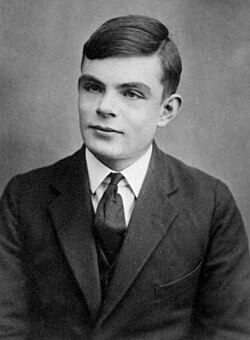
\includegraphics[width=2.5cm]{Alan_Turing.jpg}
\end{textblock*}

\begin{textblock*}{6cm}(0.2cm,5.5cm)
\begin{itemize}
    \item \textbf{앨런 튜링}  
          \newline “기계가 인간처럼 대화하면,  
          \newline \quad 지능을 가진 것이다.”  
          \newline (튜링 테스트)
\end{itemize}
\end{textblock*}


% --- John Searle: 우하단 ---
\begin{textblock*}{6cm}(8cm,5.7cm)
    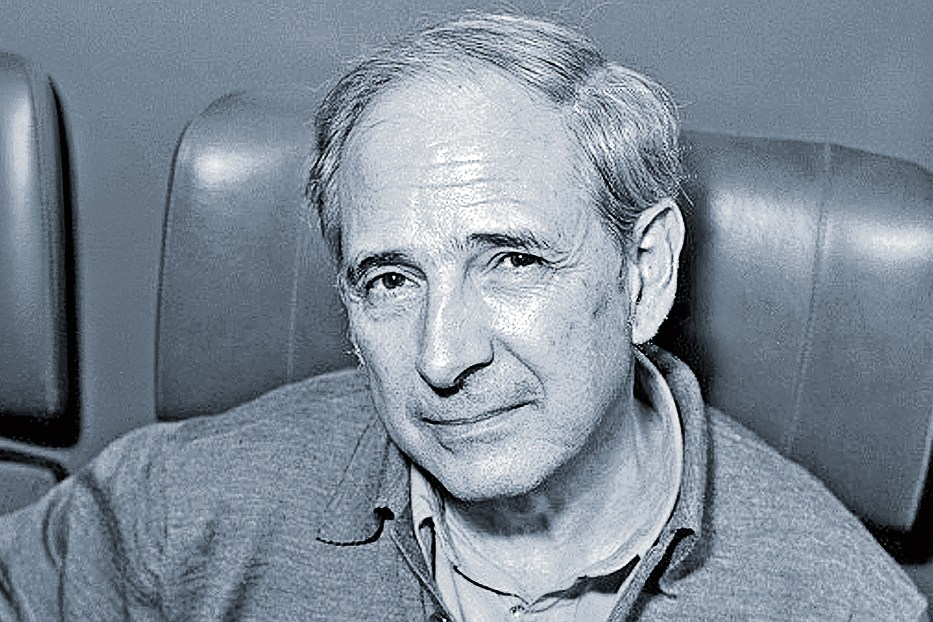
\includegraphics[width=3.5cm]{John_Searle.jpg}
\end{textblock*}

\begin{textblock*}{6cm}(7.5cm,3.2cm)
\begin{itemize}
    \item \textbf{존 설}  
          \newline “응 아니야.”  
          \newline (중국어 방 논증)
\end{itemize}
\end{textblock*}

\end{frame}
\begin{frame}{Lee Sedol and Demis Hassabis}

% --- Lee Sedol: 좌상단 ---
\begin{textblock*}{5cm}(0.8cm,1.9cm)
    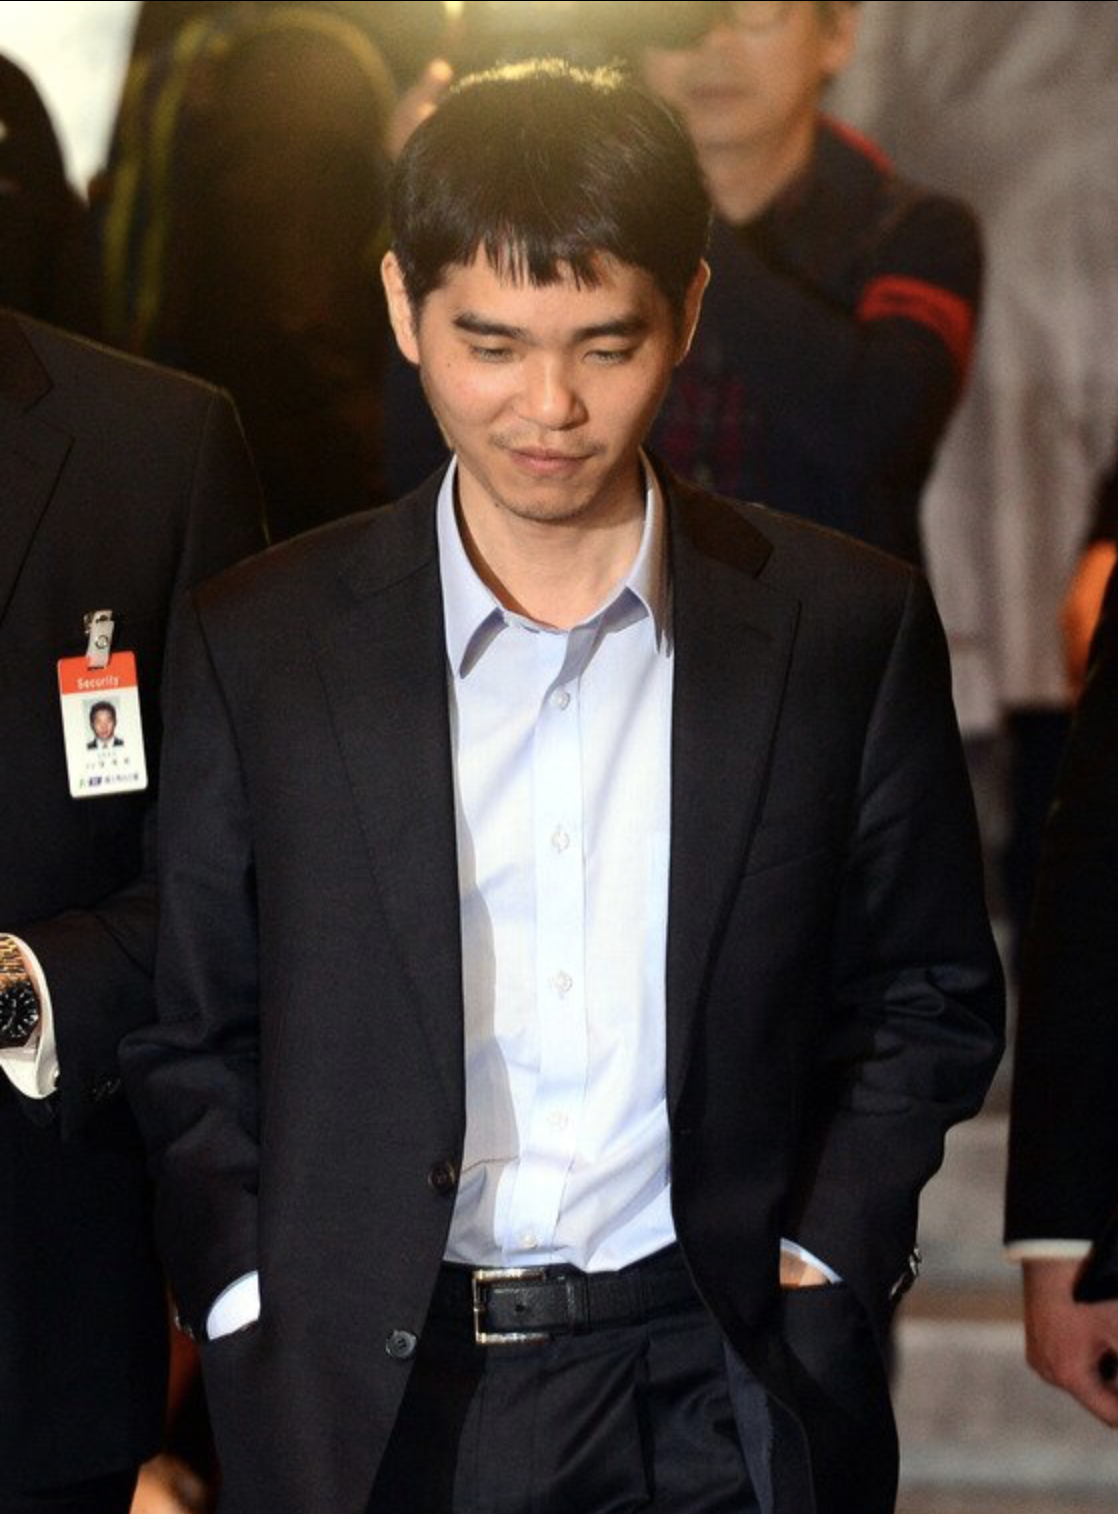
\includegraphics[width=3.2cm]{Lee}
\end{textblock*}

\begin{textblock*}{6.5cm}(0.2cm,6.5cm)
\begin{itemize}
    \item \textbf{이세돌}  
          \newline “인공지능은 완벽했다.  
          \newline \quad 하지만 완벽한 기계는 아름답지 않다.”  
\end{itemize}
\end{textblock*}


% --- Demis Hassabis: 우하단 ---
\begin{textblock*}{6cm}(8.2cm,4.2cm)
    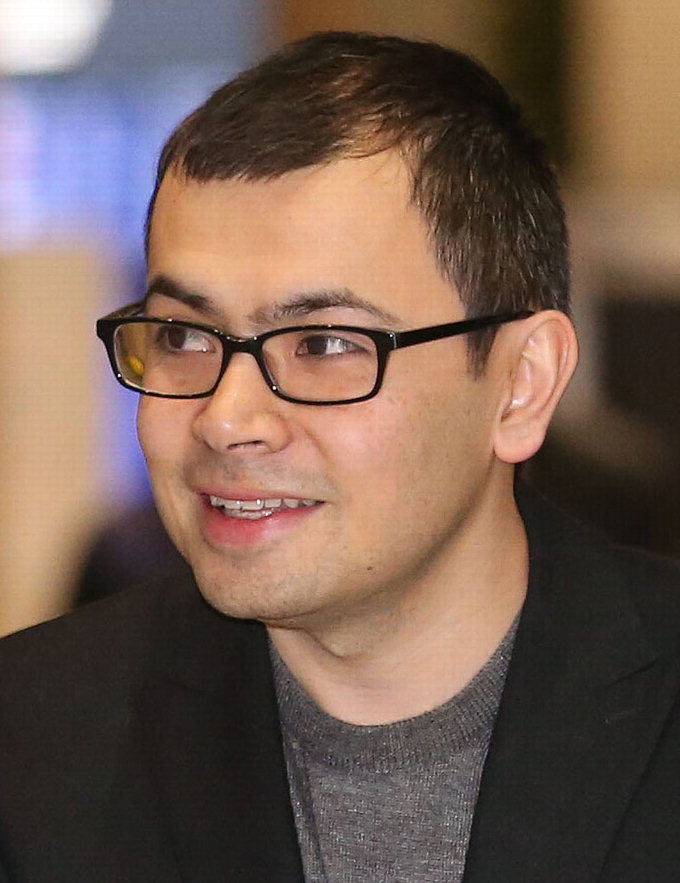
\includegraphics[width=3.2cm]{Demis_Hassabis}
\end{textblock*}

\begin{textblock*}{7cm}(7.5cm,2.3cm)
\begin{itemize}
    \item \textbf{데미스 하사비스}  
          \newline “알파고는 인간의 직관을 
          \newline \quad 배우기 시작했다.” 
\end{itemize}
\end{textblock*}

\end{frame}





\begin{frame}{AI 관련 어록}

\begin{itemize}\small

    \item 
    \begin{tabular*}{\linewidth}{@{}p{0.71\linewidth}@{\hspace{1cm}}p{0.22\linewidth}@{}}
        \textit{“기계가 생각할 수 있는지 묻기보다, 기계가 인간처럼 행동할 수 있는지 물어야 한다.”} 
        & \textbf{-앨런 튜링} \\
    \end{tabular*}

    \vspace{0.5cm}
    
    \item 
    \begin{tabular*}{\linewidth}{@{}p{0.71\linewidth}@{\hspace{1cm}}p{0.22\linewidth}@{}}
        \textit{“기호를 조작하는 것이 이해를 의미하지는 않는다.”}
        & \textbf{-존 설} \\
    \end{tabular*}

    \vspace{0.5cm}


    \item 
    \begin{tabular*}{\linewidth}{@{}p{0.71\linewidth}@{\hspace{1cm}}p{0.22\linewidth}@{}}
        \textit{“완전한 인공 지능은 인류의 종말을 의미할 수도 있다.”}
        & \textbf{-스티븐 호킹} \\
    \end{tabular*}

    \vspace{0.5cm}

    \item 
    \begin{tabular*}{\linewidth}{@{}p{0.71\linewidth}@{\hspace{1cm}}p{0.22\linewidth}@{}}
        \textit{“인공지능은 거부할 수 없는 큰 흐름이다.”}
        & \textbf{-???} \\
    \end{tabular*}

\end{itemize}

\end{frame}



\subsection{함수}
%%%%%





\begin{frame}{토의 1}
\centering
\Huge
   {함수}란 무엇인가?
\end{frame}




\begin{frame}{토의 2}
\setlength{\itemsep}{12pt} % 항목 간 간격 넉넉하게

\Huge
\centering
  우리 주변의 {함수}는 \\
  \vspace{0.3cm}
  어떤 것이 있을까?

%\centering % 중앙 정렬

%\begin{itemize}
%  \item[1.] 자판기\\[4pt]
%  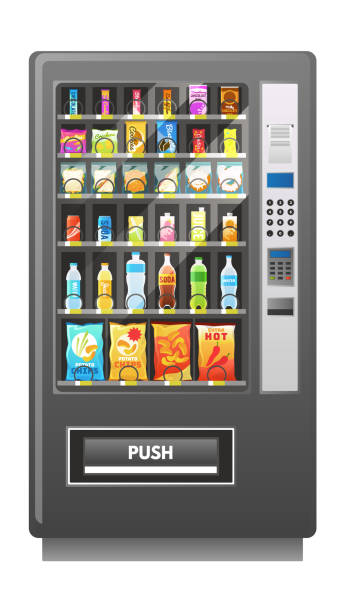
\includegraphics[width=1cm]{bending_machine.jpg}

  %\item[2.] 도어락\\[4pt]
  %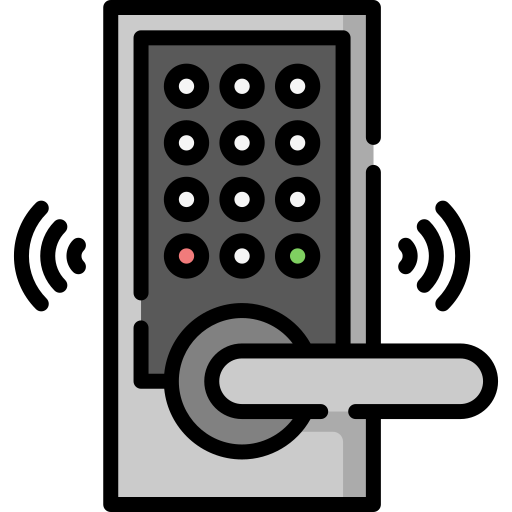
\includegraphics[width=1.2cm]{smart_lock.png}

  %\item[3.] 엘리베이터\\[4pt]
  %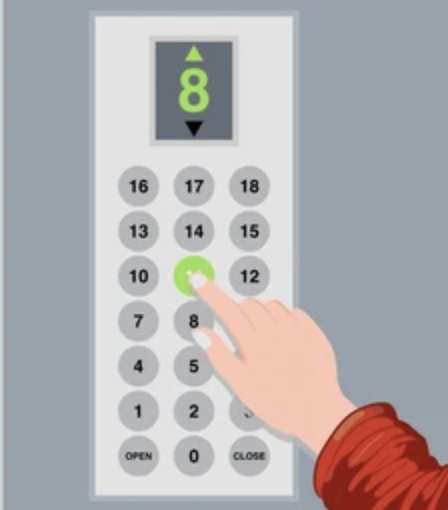
\includegraphics[width=1.4cm]{elevator_buttons}
%\end{itemize}
\end{frame}



\begin{frame}{토의 3}
\centering
\Huge
인공지능은 함수인가?    
\end{frame}




\begin{frame}{함수란?}
\centering
\Huge
   {함수}는 어디에나 있다.
\end{frame}


\begin{frame}{함수의 정의}

\begin{itemize}\setlength{\itemsep}{9pt}

    \item[1.] 두 변수 \(x, y\)에 대하여 \(x\)의 값이 하나 정해지면\\
    그에 따라 \(y\)의 값도 오직 하나로 정해지는 {\color{Sogang}{대응}}을 함수라 한다.
    \footnote{중학교 수학(일차함수 단원), 미래엔·천재교육·금성출판사}

    \item[2.] 두 집합 \(X, Y\)에서 \(X\)의 각 원소에\\
    \(Y\)의 원소가 오직 하나씩 {\color{Sogang}{대응}}할 때 이를 함수라 한다.
    \footnote{고등수학(공통수학·수학Ⅰ) 함수 단원, 미래엔·천재교육·금성출판사}

    \item[3.] 함수 \(f : X \to Y\)는\\
    정의역 \(X\)의 각 원소를 공역 \(Y\)의 한 원소에 {\color{Sogang}{대응}}시키는 규칙이다.
    \footnote{\textit{Principles of Mathematical Analysis} (Walter Rudin, 3rd ed., 1976)}

\end{itemize}

\end{frame}


\section{선형 회귀}


\subsection{소행성 세레스}


\begin{frame}{Ceres and Piazzi}


\begin{textblock*}{5cm}(0.8cm,1.9cm)
    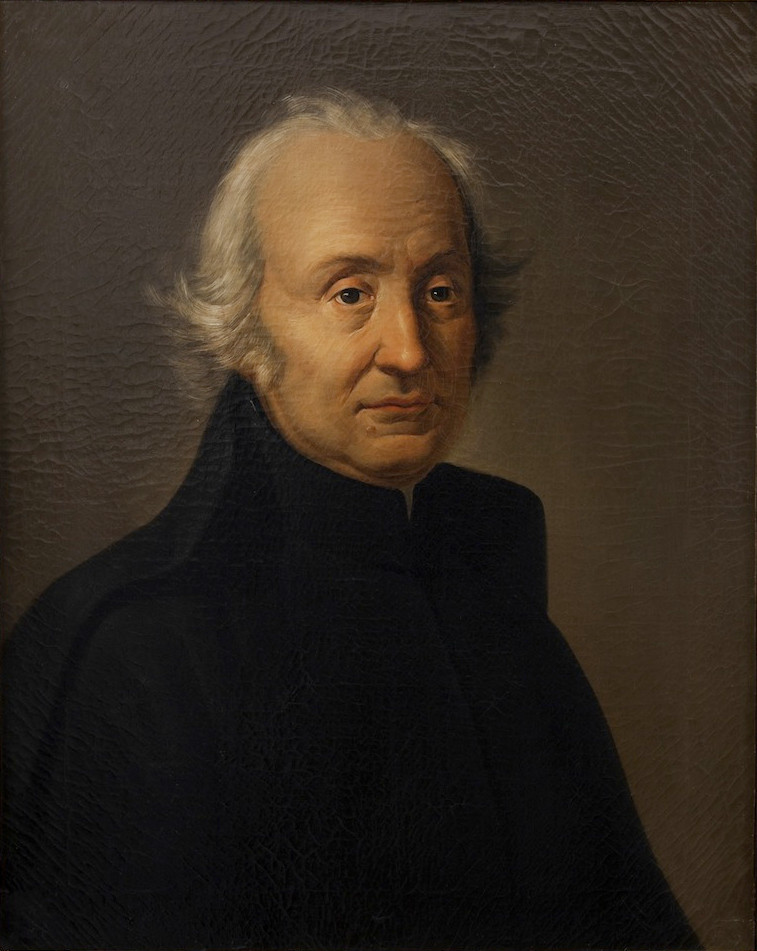
\includegraphics[width=3.2cm]{piazzi.jpg}
\end{textblock*}

\begin{textblock*}{6.5cm}(0.2cm,6.5cm)
\begin{itemize}
    \item \textbf{피아치}  
          \newline 새로운 행성 발견한거 같은데? 
          \newline 관측하다가 놓쳐버렸넹..
          \end{itemize}
\end{textblock*}







\begin{textblock*}{7cm}(8.2cm,1.7cm)
    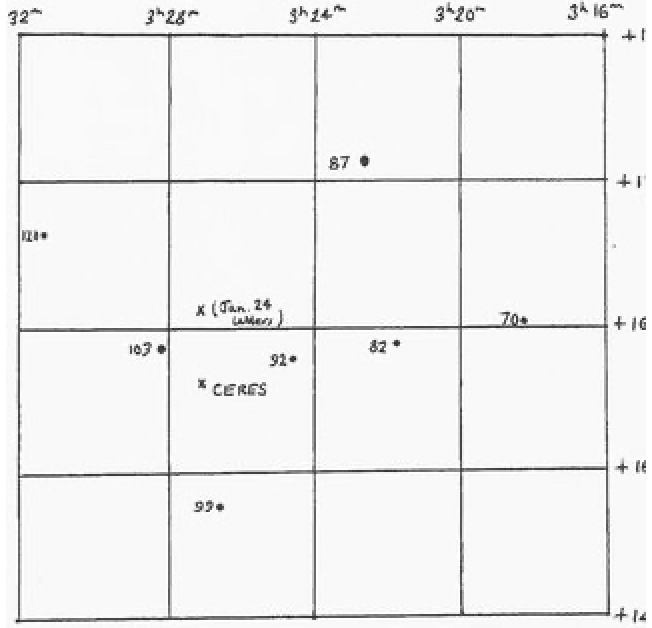
\includegraphics[width=3.2cm]{Ceres_observation.png}
\end{textblock*}

\begin{textblock*}{6cm}(8.2cm,5.3cm)
    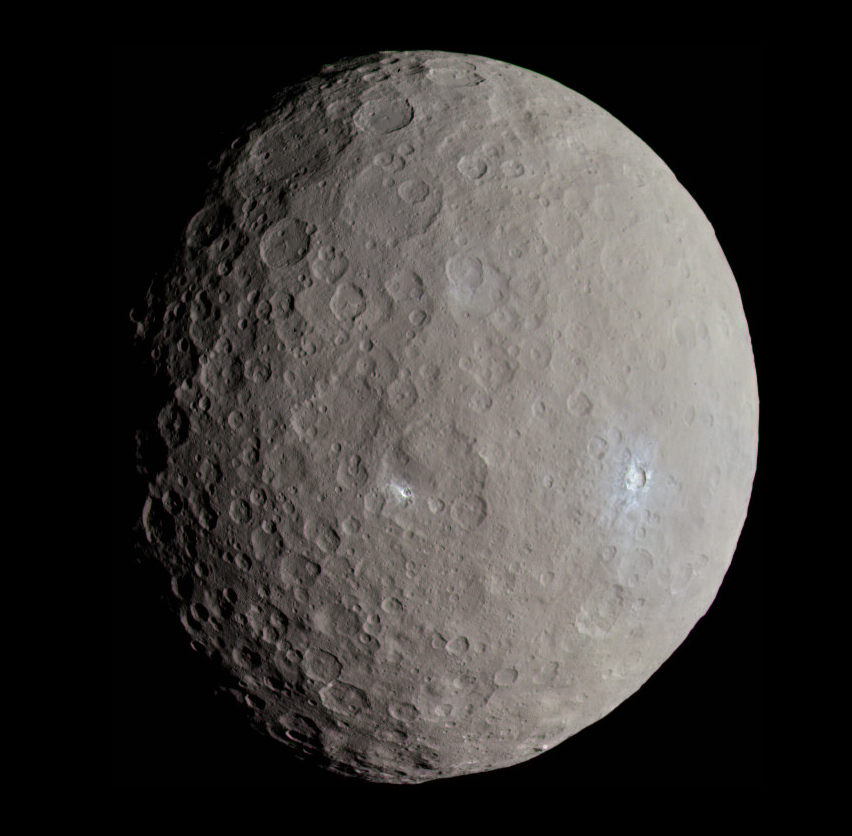
\includegraphics[width=3.2cm]{Ceres.jpg}
\end{textblock*}

\end{frame}



\begin{frame}{Gauss}


\begin{textblock*}{5cm}(0.8cm,1.9cm)
    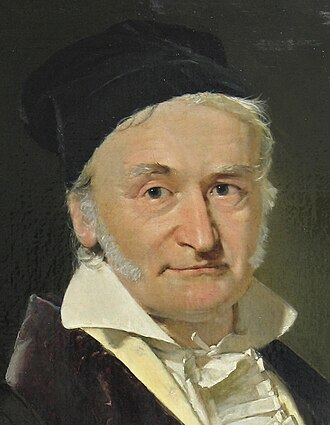
\includegraphics[width=3.2cm]{Gauss.jpg}
\end{textblock*}

\begin{textblock*}{6.5cm}(0.2cm,6.5cm)
\begin{itemize}
    \item \textbf{가우스}  
          \newline 관측값의 \textbf{오차제곱합}을 줄이면 될거같은데?
\end{itemize}
\end{textblock*}

\begin{textblock*}{6cm}(6.2cm,2.3cm)
    \begin{itemize}
    \item \textbf{최소제곱법}  
          \newline 오차제곱합을 최소화 하는 방식으로 궤도 계산에 성공\footnote{Theoria Motus Corporum Coelestium in Sectionibus Conicis Solem Ambientium}.
          \newline
          \newline 가우스가 지정한 날짜와 장소에서 세레스 관측 성공!
\end{itemize}
\end{textblock*}

\end{frame}


\subsection{최소제곱법}

\begin{frame}{최소제곱법}
    
\centering
\Large
주어진 데이터를 \textcolor{Sogang}{가장 잘 설명하는 직선}을 찾는 방법.
\end{frame}

\begin{frame}{데이터와 직선 (1)}

\centering
    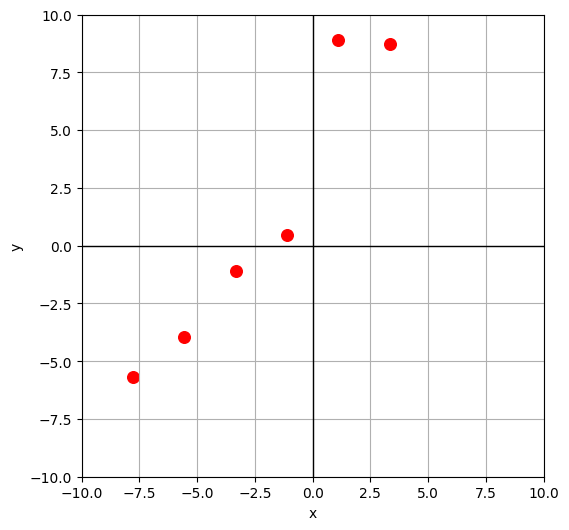
\includegraphics[width=8cm]{points.png}
\end{frame}


\begin{frame}{데이터와 직선 (2)}

\centering
    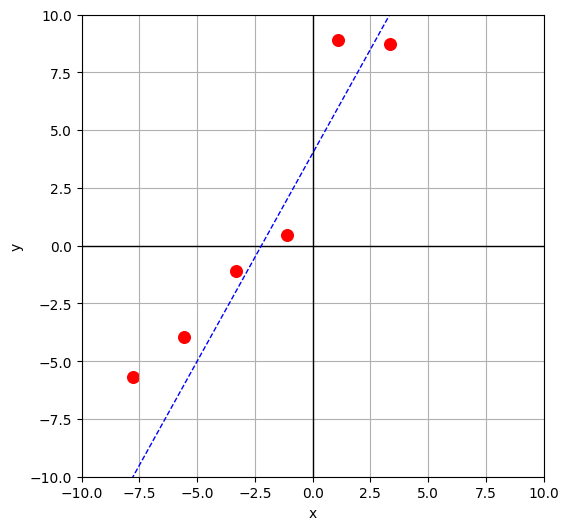
\includegraphics[width=8cm]{line.png}
\end{frame}




\begin{frame}{데이터와 직선 (3)}

\centering
    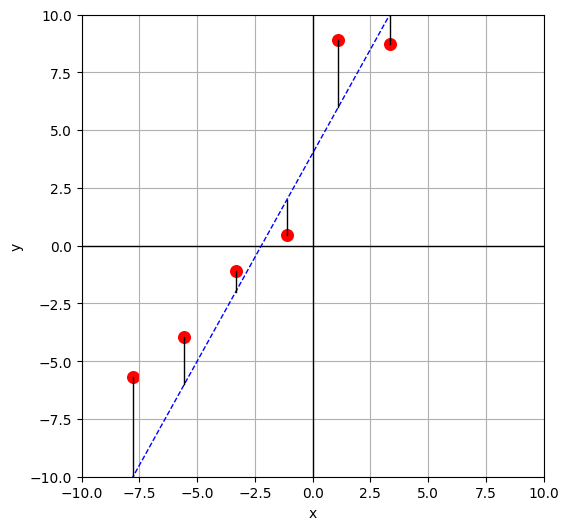
\includegraphics[width=8cm]{error.png}
\end{frame}


\begin{frame}{일차 함수와 오차}

\begin{itemize}
    \item 주어진 데이터:
    \newline
    \small{
    $
    (-7.8, -5.7),\;
    (-5.6, -3.9),\;
    (-3.3, -1.1),\;
    (-1.1, 0.5),\;
    (1.1, 8.9),\;
    (3.3, 8.8)
    $
    }
    \newline

    \item 직선의 방정식:
    \[
        y = ax + b
    \]

    \item 오차 계산:
    \[
    \begin{aligned}
        r_1 &= -5.7 - (a(-7.8) + b), \\
        r_2 &= -3.9 - (a(-5.6) + b), \\
        r_3 &= -1.1 - (a(-3.3) + b), \\
        r_4 &= 0.5  - (a(-1.1) + b), \\
        r_5 &= 8.9  - (a(1.1)  + b), \\
        r_6 &= 8.8  - (a(3.3)  + b).
    \end{aligned}
    \] 
    \item 가우스의 아이디어: 
    \newline
    \textbf{제곱}의 합 $r_1^2+\dots+r_6^2$ 을 최소로 만드는 $a$와 $b$를 찾자!

\end{itemize}

\end{frame}


\begin{frame}{최소제곱법: $a$와 $b$ 구하기}

\begin{itemize}

    \item 오차제곱합:
    \[
    \begin{aligned}
        S(a,b)
        &= r_1^2 + \dots + r_6^2\\
        &= (-5.7 - (a(-7.8) + b))^2 + \cdots + (8.8 - (a(3.3) + b))^2.
    \end{aligned}
    \]

    \item $S(a,b)$는 $a$와 $b$를 넣으면 값이 정해지는 \textbf{함수}이다.

    \item[$\nabla$] 이 함수는 \emph{미분}이 가능하고, \emph{아래로 볼록(convex)}하다.

    \item[$\nabla$] 따라서 $a$와 $b$에 대해 각각 \emph{편미분}하여
    \[
        \frac{\partial S}{\partial a} = 0, \qquad
        \frac{\partial S}{\partial b} = 0
    \]
    을 만족하는 해를 구할 수 있다.

\end{itemize}

\end{frame}


\begin{frame}{$S(a,b)$의 그래프}

\begin{itemize}
    \item $S(a,b)
=
116.4a^2
-26.8ab
+6b^2
-216.42a
-15b
+205.81$
\item  $a=1.44$, $b=4.48$.
 
\end{itemize}
  
  \centering
    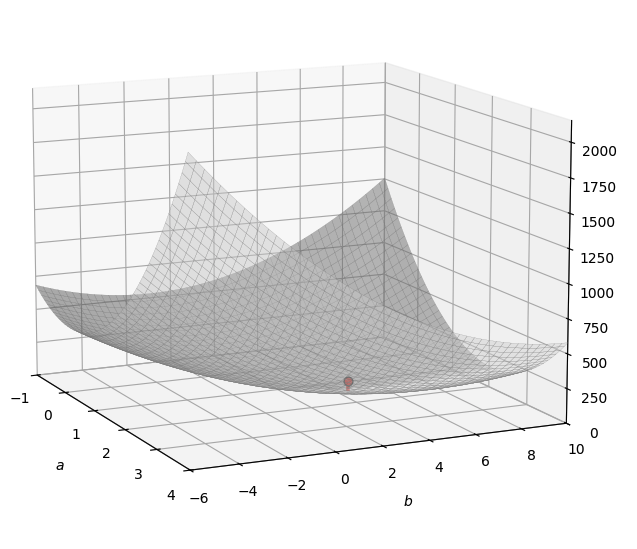
\includegraphics[width=8cm]{figure_s(a,b).png}  
\end{frame}




\begin{frame}{데이터와 직선 (4)}

\centering
    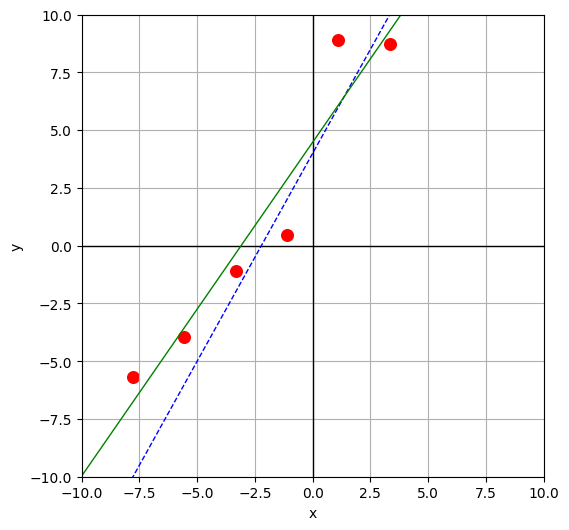
\includegraphics[width=8cm]{LSE.png}
\end{frame}






\begin{frame}


\centering
\Huge
  감사합니다

\begin{textblock*}{5cm}(7cm,8cm) % {width}(x,y) - adjust x and y as needed

\includegraphics[scale=0.2]{minds}
\end{textblock*}
%%%%%



\end{frame}














\end{document}